\chapter{Evolutionary dynamics on graphs}
\label{chp:nature} 
\cite{lieberman2005evolutionary}
Tanker fra paper:

If advantegous mutant(f.eks virus) incerted in circulation graph, it will have a fixation probability 
\begin{equation}  p_{1}=\frac{(1-1/r)}{(1-1/r^{N})} \label{eq:fixation} \end{equation}
Isotherm graphs are a subgraph of circulation. 

If $W$ is symmetric, or isotherm then the fixation probability is allways \ref{eq:fixation}
isotherm means doubly stochastic, all rows and cols sum to 1. 
If a graph is one rooted, it has a fixation prob of $1/N$ regardless of $r$. If a graph has more then one root, its fixation probability is zero. 
Is it possible to find graphs with fixation probability that exceeds \ref{eq:fixation}? Is it possible to suppress drift and amplify selection?
In a star-topology \ref{fig:star} the fixation probability is\begin{equation}p_{2}=\frac{(1-1/r^{2})}{(1-1/r^{2N})} \label{eq:fixation2} \end{equation}.
or more generally: \begin{equation}
p_{k}=\frac{(1-1/r^{k})}{(1-1/r^{kN})} \label{eq:fixationk}
\end{equation}
And the selective difference is as we see amplified from $r$ to $r^{2}$. i.e. a star act as an evolutionary amplifier,
 favouring advantageous mutants and inhibiting disadvantageous mutants, tilts towards selection and against drift.
 in certain graphs, star, funnel, metafunnel, if N is large enough, fixation proability for advantageous mutant converges to 1. Fixprob for disadvantaeus converges to 0.
This could maybe be used to show that if we have a star, funnel, metafunnel or something, and we secure the nodes it could force the virus to die out?
Scale-free networks have most of their connectivity clustered in a few vertices, i.e. they are potent selection amplifiers.
More generalized, $W$ does not need to be stochastic, $w_{ij}>=0$. 
If the sum of all edges leaving a vertex is equal for all vertexes, then the graph will never suppress selection.
If the sum of all edges entering a vertex is equal for all vertexes, the graph never suppress drift.
If both then the graph is called a circulation.
 
The game:
The way this game works, is that we look at nodes that are mutated (A), and those who are not (B). When we apply the game to a directed graph, there are four different outcomes, a,b,c and d, which represents the interaction between the nodes, as is depicted in the figures below. (BRUK figurer fra paperet). The fixation probability is related to r=b/c in the first figure (Positive symmetric). If b is greater than c, the properties of mutant b will “propagated” in to all the other nodes, and the whole graph will eventually consists of only mutated nodes. The opposite will happen in the case where c is greater than b, leading to extinction of the mutation. 


\begin{figure}
\centering
\begin{tabular}{@{}c@{}}
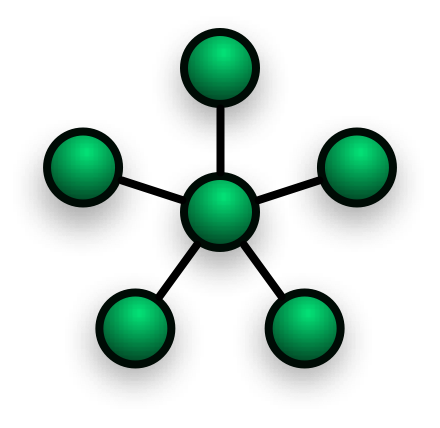
\includegraphics[width=0.5\textwidth]{NetworkTopology-Star.png}
\end{tabular}
\caption{\label{fig:star} A star-topology}
\end{figure}



